\documentclass[12pt]{article}
\usepackage{graphicx} % Required for inserting images
\usepackage[letter, margin=0.5in]{geometry}
\usepackage{amsmath, mathrsfs, amssymb, cancel, tikz} % for various mathematical symbols
\usetikzlibrary{patterns, shapes.geometric}


\graphicspath{{./images/}}

\setcounter{secnumdepth}{0} % Removes section numbering

\usepackage{titling}
\renewcommand\maketitlehooka{\null\mbox{}\vfill}
\renewcommand\maketitlehookd{\vfill\null}

\title{Physical Mechanics Homework 10}
\date{12/05/2024}
\author{Damien Koon}


\documentclass[tikz,border=2mm]{standalone}


\begin{document}

\maketitle

\newpage
\textbf{TM 2-41 A train moves along the tracks at a constant speed u. A woman on the train throws a ball of mass m straight ahead at a speed v with respect to herself.}

\textit{
(a) What is the kinetic energy gain of the ball as measured by a person on the train?}

\textit{
(b) What is the kinetic energy gain of the ball as measured by a person standing by the railroad
tracks?}

\textit{
(c) How much work is done by the woman throwing the ball?}

\textit{
(d) How much work is done by the train?
} \newline

\begin{center}
    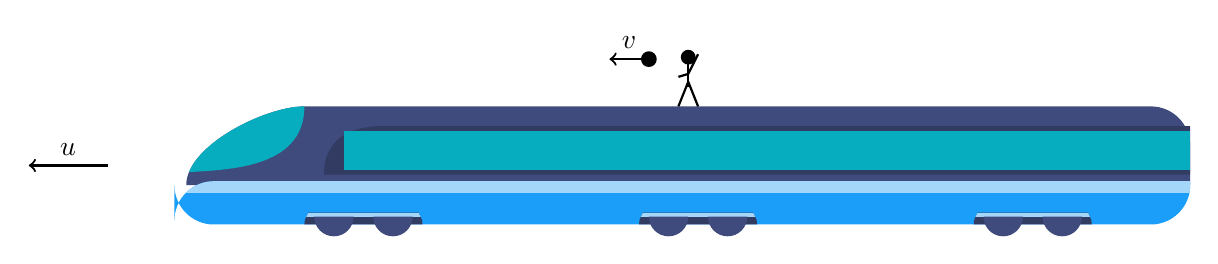
\begin{tikzpicture}[
        scale = 0.5,
        declare function = {%
            windshieldupx(\x)   = {6*(1 - \x)*\x*\x + 3*\x*\x*\x};
            windshieldupy(\x)   = {3*(1 - \x)*(1 - \x)*\x + 6*(1 - \x)*\x*\x + 2*\x*\x*\x};
            windshielddownx(\x) = {3*(1 - \x)*(1 - \x)*(1 - \x) + 9*(1 - \x)*(1 - \x)*\x + 3*(1 - \x)*\x*\x + windshieldupx(0.11)*\x*\x*\x};
            windshielddowny(\x) = {2*(1 - \x)*(1 - \x)*(1 - \x) + 3*0.4*(1 - \x)*(1 - \x)*\x + 3*0.4*(1 - \x)*\x*\x + windshieldupy(0.11)*\x*\x*\x};
        }
    ]
    
        \definecolor{window}{RGB}{5,173,190}
        \definecolor{trainbody}{RGB}{64,75,125}
        \definecolor{aroundwindow}{RGB}{50,59,97}
        \definecolor{bottomtrain}{RGB}{27,158,249}
        \definecolor{trainline}{RGB}{164,214,249}
        
        \tikzset{%
            trainwindow/.style = {%
                rectangle,
                fill           = window,
                draw           = none,
                minimum width  = 1cm,
                minimum height = 0.5cm
            }
        }
            
        \newcommand{\trainlength}{25.5}
                    
        \fill[
            trainbody
        ] plot[domain = 0:1, samples = 100] ({windshieldupx(\x)},{windshieldupy(\x)}) {%
            [rounded corners = 0.5cm]
                -- (\trainlength, 2)
        }
            -- ++(0, -2) -- cycle;
            
        \fill[%
            fill = window
        ] plot[domain = 0.11:1, samples = 100] ({windshieldupx(\x)},{windshieldupy(\x)})
            plot[domain = 0:1, samples = 100] ({windshielddownx(\x)},{windshielddowny(\x)})
            -- ({windshieldupx(0.11)},{windshieldupy(0.11)})
            -- cycle;
    
        \fill[%
            aroundwindow
        ] (3.5, {windshieldupy(0.09)}) .. controls (3.5, 0.5) and (3.5, 1.5) .. (5, 1.5)
            -- (\trainlength, 1.5)
            -- (\trainlength, {windshieldupy(0.09)})
            -- cycle;
    
        \foreach \x in {5,6.5,...,\trainlength} {
            \node[trainwindow] at (\x, {(windshieldupy(0.09) + 1.5)/2}) {};
        }
    
        \fill[%
            bottomtrain
        ] {%
            [rounded corners = 0.5cm]
            (\trainlength, 0.1) 
                -- (\trainlength, -1)
                -- (-0.3, -1)
                -- (-0.3, 0.1)}
            -- cycle;
            
        \begin{scope}
        
            \path[clip] {%
                [rounded corners = 0.5cm]
                (\trainlength, 0.1) 
                -- (\trainlength, -1)
                -- (-0.3, -1)
                -- (-0.3, 0.1)}
            -- cycle;
            
            \fill[trainline] (-0.3, -0.2) rectangle (\trainlength, 0.1);
            
        \end{scope}
    
        \foreach \x in {3, 11.5, 20} {
    
            \fill[
                aroundwindow
            ] (\x, -1) .. controls (\x, -0.9) and (\x, -0.9) .. ({\x + 0.1}, -0.7)
                -- ({\x + 2.9}, -0.7) .. controls ({\x + 3}, -0.9) and ({\x + 3}, -0.9) .. ({\x + 3}, -1)
                -- cycle;
        
            \begin{scope}
            
                \path[clip] (\x, -1) .. controls (\x, -0.9) and (\x, -0.9) .. ({\x + 0.1}, -0.7)
                    -- ({\x + 2.9}, -0.7) .. controls ({\x + 3}, -0.9) and ({\x + 3}, -0.9) .. ({\x + 3}, -1)
                    -- cycle;
                
                \fill[trainline] (\x, -0.8) rectangle ({\x + 3}, -0.7);
            
            \end{scope}
            
            \fill[%
                trainbody
            ] ({\x + 0.25}, -0.8) arc (-180:0:0.5); 
        
            \fill[%
                trainbody
            ] ({\x + 1.75}, -0.8) arc (-180:0:0.5); 
    
        }

    % Stick figure on top of the train
    \draw[thick] (\trainlength/2, 2.5*1.25) -- ++(0, -0.5*1.25); % Body
    \draw[thick] (\trainlength/2, 2.5*1.25 - 0.3) -- ++(0.25, 0.5); % Left arm raised,
    \draw[thick] (\trainlength/2 - 0.2*1.25, 2.2*1.25) -- (\trainlength/2, 2.5*1.25 - 0.3); % Right arm
    \draw[thick] (\trainlength/2, 2.5*1.25 - 0.5) -- ++(-0.2*1.25, -0.5*1.25); % Left leg
    \draw[thick] (\trainlength/2, 2.5*1.25 - 0.5) -- ++(0.2*1.25, -0.5*1.25); % Right leg
    \fill (\trainlength/2, 2.6*1.25) circle (0.15*1.25); % Head

    \fill (\trainlength/2 - 1, 3.2) circle (0.2); % Ball to the left of the person
    \draw[->, thick] (\trainlength/2 - 1, 3.2) -- ++(-1, 0) node[midway, above] {\(v\)}; % Velocity vector

    \draw[->, thick] (-2, 0.5) -- ++(-2, 0) node[midway, above] {\(u\)};

    \end{tikzpicture}
\end{center}

$$
\boldsymbol{T_{Person} = T_f - t_i = \frac{1}{2}mv^2}
$$

$$
T_{observer} = T_f - T_i = \frac{1}{2}m(v+u)^2 - \frac{1}{2}mu^2
$$

$$
\boldsymbol{T_{observer} = \frac{1}{2}mv^2 + mvu}
$$

$$
\boldsymbol{W_{woman} = \Delta T_{person} = \frac{1}{2}mv^2}
$$

$$
\boldsymbol{W_{train} = T_{observer} - T_{woman} = mvu}
$$


\newpage
\textbf{TM 2-47 Consider a particle moving in the region $x > 0$ under the influence of the potential
}

$$
\boldsymbol{U(x) = U_0 (\frac{a}{x} + \frac{x}{a})}
$$

\textit{Where $U_0 = 1 J$ and $a = 2 m$} \newline

\textit{
(a) Sketch the potential.}

\textit{
(b) Find the equilibrium point(s).}

\textit{
(c) Determine whether each point found in part (b) represents a stable or an unstable equilibrium.}

\begin{center}
\begin{tikzpicture}
    % Define the axes
    \draw[->] (-0.5, 0) -- (6, 0) node[right] {$x$};
    \draw[->] (0, -0.5) -- (0, 6) node[above] {$U(x)$};

    % Plot the function
    \begin{scope}
        \clip (-0.5, -0.5) rectangle (6, 6); % Clip the function to stay within axes
        \draw[domain=0.2:6, samples=200, smooth, thick, blue] 
            plot (\x, {2/\x + \x/2});
    \end{scope}
    
    % Add labels
    \node[below left] at (0, 0) {0};
    \node[below] at (2, 0) {$a=2m$};
    
    % Add a dotted line to show the minimum point
    \draw[dashed, gray] (2, 0) -- (2, 2) node[above right] {$\left(2, \, 2\right)$};
    \draw[dashed, gray] (0, 2) -- (2, 2);
\end{tikzpicture}
\end{center}

$$
U(x) = U_0 (\frac{a}{x} + \frac{x}{a})
$$

$$
\frac{d}{dx} U(x) = \frac{d}{dx} U_0(-\frac{a}{x^2} + \frac{1}{a}) = U_0(-\frac{a}{x^2} + \frac{1}{a}) = 0
$$

Ignoring -2 because $x > 0$
$$
\therefore x = \pm 2 \rightarrow \boldsymbol{x = 2}
$$

$$
\frac{d^2}{dx^2} U(x) \mid_{x=2} = \frac{d^2}{dx^2} U_0 (\frac{a}{x} + \frac{x}{a}) \mid_{x=2} = U_0 ( \frac{2a}{x^3})\mid_{x=2} = \frac{1}{4} U_0 a > 0
$$

$$
U_0, a > 0 \rightarrow \frac{d^2}{dx^2} U(x) > 0
$$

$$
\boldsymbol{\therefore \exists \textit{ a stable equilibrium at the point } x =2}
$$


\newpage
\textbf{TM 7-26 Determine the Hamiltonian and Hamilton’s equations of motion for}

\textit{
(a) a simple pendulum of length ℓ and bob mass m (hint: do not assume small angles)
}

\textit{
(b) a simple Atwood’s machine with a single pulley and a massless string
}

% Part a
\begin{center}
\begin{tikzpicture}

% Mass 1
\draw[thick] (-1.49cm,0) -- ++(0,-3.5cm) node[draw=black,above=0.13cm,circle,fill=brown!70!black](cm){} node[draw=black,trapezium,rounded corners=1pt,fill=brown!70!black,text=white, minimum height=0.6cm](m){$m_1$};

% Mass 2
\draw[thick] (1.49cm,0) -- ++(0,-5cm) node[draw=black,above=0.18cm,circle,fill=brown!70!black](cM){}
node[draw=black,trapezium,rounded corners=1pt,fill=brown!70!black,text=white, minimum height=0.7cm](M){$m_2$};

% Supporting structure
\fill[pattern= north west lines,] (-2.5,2.41) rectangle (2.5,2.6);
\draw(-2.5,2.41) -- (2.5,2.41);

% Pulley
\draw[fill = gray] (0,0) circle (1.5cm); % Big circle
\draw[fill=lightgray] (0,0) circle (1.3cm); % Medium circle
\draw[fill=white] (75:2.5) to[rounded corners=0.2cm] (0.2,-0.25)
to[rounded corners=0.2cm] (-0.2,-0.25) -- (105:2.5) -- cycle;
\draw[fill=darkgray] (0,0) circle (0.12cm); % Axle circle

% Dotted line for m_1 
\draw[dotted] (-3,0) -- (-3,-3.5) node[x, above=1.75cm]{x};

% Dotted line for m_2
\draw[dotted] (3,0) -- (3,-5) node[y, above=2.25cm]{y};


\end{tikzpicture}
\end{center}

$$
\ell = x + y + 2\pi \rightarrow x = x, \quad y = \ell - x - 2\pi
$$

$$
T = \frac{1}{2}m_1 \dot{x}^2 + \frac{1}{2}m_2 \dot{x}^2
$$

$$
U = -m_1gx -m_2g(\ell - x - 2 \pi) 
$$

$$
\mathscr{L} = \frac{1}{2}m_1 \dot{x}^2 + \frac{1}{2}m_2 \dot{x}^2 + m_1gx + m_2g(\ell - x - 2 \pi) 
$$

$$
P_x = \frac{d \mathscr{L}}{d\dot{x}} =  (m_1 + m_2) \dot{x}
$$

$$
H = T + U = \frac{1}{2}m_1 \dot{x}^2 + \frac{1}{2}m_2 \dot{x}^2 -m_1gx - m_2g(\ell - x - 2 \pi)
$$

$$
H = \frac{P_x^2}{2(m_1 + m_2)} -m_1gx - m_2g(\ell - x - 2 \pi)
$$

$$
\dot{x} = \frac{dH}{dP_x} \rightarrow P_x = (m_1 + m_2) \dot{x}
$$

$$
-\dot{P_x} = \frac{dH}{dx} \rightarrow (m_1 + m_2) \ddot{x} = (m_1 - m_2)g
$$

$$
\boldsymbol{\ddot{x} = g \frac{m_1 + m_2}{m_1 - m_2}}
$$


\newpage
% Part b
\begin{center}
\begin{tikzpicture}
    % Draw axes
    \draw[->] (0,0) -- (0,0.5) node[above] {$y$};
    \draw[->] (0,0) -- (0.5,0) node[right] {$x$};

    % Draw vector
    \draw[->,thick] (0,0) -- (1.5,-1.5) node[below right] {$m$};

    % Draw length, l
    \node at (1, -0.75) {$\ell$};

    % Draw dotted line
    \draw[dotted] (0,0) -- (0, -2)
    \node at (-0.3, 0) {$O$};

    % Draw angle theta
    \draw[thick] (0,-0.5) arc[start angle=-90, end angle=-45, radius=0.5];
    \node at (0.3,-0.8) {$\theta$};

    % Draw circle at the end of vector
    \draw[thick] (1.5,-1.5) circle (0.1);
\end{tikzpicture}
\end{center}

$$
x = \ell \sin \theta, \quad y = -\ell \cos \theta
$$

$$
\dot{x}^2 + \dot{y}^2 = \cancel{\dot{\ell}^2} + \ell^2 \dot{\theta}^2
$$

$$
T = \frac{1}{2} m \ell^2 \dot{\theta}^2, \quad U = -m g \ell \cos \theta
$$

$$
\mathcal{L} = T - U = \frac{1}{2} m \ell^2 \dot{\theta}^2 + m g \ell \cos \theta
$$

$$
P_\theta = \frac{\partial \mathcal{L}}{\partial \dot{\theta}} = m \ell^2 \dot{\theta}
$$

$$
\dot{P}_\theta = \frac{d}{dt} P_\theta = m \ell^2 \ddot{\theta}
$$

$$
H = T + U = \frac{1}{2} m \ell^2 \dot{\theta}^2 - m g \ell \cos \theta
$$

$$
P_{\theta} = m \ell^2 \dot{\theta}
$$

$$
H = \frac{P_{\theta}^2}{2m \ell^2} - m g \ell \cos \theta
$$

$$
\dot{\theta} = \frac{dH}{dP_{\theta}} \rightarrow P_{\theta} = m \ell^2 \dot{\theta}
$$

$$
- \dot{P_{\theta}} = \frac{dH}{d\theta} \rightarrow -m \ell^2 \ddot{\theta} = mg\ell sin(\theta)
$$

$$
m \ell^2 \ddot{\theta} + m g \ell \sin \theta = 0
$$

$$
\boldsymbol{\ddot{\theta} + \frac{g}{\ell} \sin \theta = 0}
$$


\newpage
\textbf{TM 7-41 A pendulum of length b and bob mass m is oscillating at small angles when
the length of the pendulum string is shortened at a velocity of $\alpha$ (i.e. $\frac{db}{dt} = \alpha$). Find Lagrange’s equations of motion. (Hint: since the oscillation is very small, the string is very
nearly vertical.)}

\begin{center}
\begin{tikzpicture}
    % Draw axes
    \draw[->] (0,0) -- (0,0.5) node[above] {$y$};
    \draw[->] (0,0) -- (0.5,0) node[right] {$x$};

    % Draw vector
    \draw[->,thick] (0,0) -- (1.5,-1.5) node[below right] {$m$};

    % Draw length, l
    \node at (1, -0.75) {$b$};

    % Draw dotted line
    \draw[dotted] (0,0) -- (0, -2)
    \node at (-0.3, 0) {$O$};

    % Draw angle theta
    \draw[thick] (0,-0.5) arc[start angle=-90, end angle=-45, radius=0.5];
    \node at (0.3,-0.8) {$\theta$};

    % Draw circle at the end of vector
    \draw[thick] (1.5,-1.5) circle (0.1);
\end{tikzpicture}
\end{center}

$$
T = \frac{1}{2}m\dot{b}^2 + \frac{1}{2}mb^2\dot{\theta}^2 
$$

$$
U = -mgbcos(\theta)
$$

$$
\mathscr{L} = \frac{1}{2}m\dot{b}^2 + \frac{1}{2}mb^2(\dot{\theta})^2 + mgbcos(\theta)
$$

$$
\frac{\partial \mathscr{L}}{\partial b} - \frac{d}{dt}\frac{\partial \mathscr{L}}{\partial \dot{b}} = 0 
$$

$$
\boldsymbol{b\dot{\theta}^2 - gcos(\theta) \dot{\alpha} = 0}
$$

$$
\frac{\partial \mathscr{L}}{\partial \theta} - \frac{d}{dt}\frac{\partial \mathscr{L}}{\partial \dot{\theta}} = 0 
$$

$$
\boldsymbol{
2 \alpha \dot{\theta} + b \ddot{\theta} + \frac{g}{b}sin(\theta) = 0
}
$$

\end{document}
